\chapter{Analyse}
\label{ch:analyse}

Um die Effizienz des implementierten Verfahrens bewerten zu können wurde es einer umfangreichen Evaluierung unterzogen. Die Ergebnisse sind in diesem Kapitel gesammelt. 

\section{Hörbarkeit}

Die Resultate werden von der Implementierung immer mit den Tools EAQUAL und PQevalAudio bewertet. Dabei hat sich gezeigt, dass der berechnete ODG\index{Objective Difference Grade} bei einer $\mbox{esf}=1$ meistens kleiner $-3$ liegt, wobei PQevalAudio traditionell etwas schlechter bewertet. Per Definition des PEAQ\index{Perceptual Evaluation of Audio Quality} Standards werden Werte kleiner $-2$ als \glqq{}Slightly annoying\grqq{} eingestuft und ab $-3$ gelten die Signalveränderungen als \glqq{}Annoying\grqq{}. Subjektive Hörtests mit verschiedenen handelsüblichen Kopfhörern wie sie etwa bei Smartphones beiliegen bestätigen diese Einschätzungen. Über Laptop oder PC Lautsprecher sind die Watermarks hingegen selten bis gar nicht wahrzunehmen. 

Dennoch ist in diesen Fällen eine Reduktion der Embedding Strength\index{Embedding Strength} über den Embedding Strength Factor\index{Embedding Strength Factor} (esf) vorgesehen. Jedoch hat sich ebenfalls gezeigt, dass eine interative Reduktion des esf um 10\% kaum eine Auswirkung auf die resultierenden ODGs hat.

\section{Stirmark Benchmarks}

Lange war es ein Problem verschiedene Watermarkingverfahren miteinander zu vergleichen, da die Kriterien nach denen die Robustheit getestet wurde von jedem Entwickler selbst definiert wurden. Es fehlte ein entsprechender Standard. Zu diesem Zweck wurden Anfang des neuen Jahrtausends die sog. \textit{StirMark Benchmarks}\index{Stirmark Benchmark} definiert\cite{petitcolas2000watermarking}\cite{petitcolas2004stirmark}, die derzeit in der Version 4.0 vorliegen. Dabei handelt es sich um ein definiertes Set an Angriffsverfahren\index{Angriffverfahren} die auf markierte Daten angewendet werden können. Eine Auswertung der so bearbeiteten Daten und ein Vergleich mit dem Original erlaubt Rückschlüsse auf die Stärken und Schwächen eines Watermarkingalgorithmuses, besonders auf verschiedene Angriffsfamilien (wie wir noch sehen werden), sowie eine Vergleich mit anderen Watermarkingverfahren. Jedoch werden nicht alle Angriffsszenarien welche testenswert wären auch definiert und bereitgestellt\cite{steinebach2002stirmark}.

Für die Auswertung von Audiodaten gibt es eine dedizierte \textit{Stirmark for Audio} Version\cite{stirmarkforaudio} (aktuelle v1.3.2). Auf deren Verwendung wir kurz in Anhang \ref{ch:stirmarkaudio} eingegangen, da sie sich als nicht ganz einfach herausstellen kann. Unter anderem bestehen Voraussetzungen an die Maschine, weswegen auch Bestrebungen existierten die Applikation als Cloud Service zu abstrahieren\cite{petitcolas2001public}. Eine Umsetzung dieser ist jedoch nicht abzusehen. 

Eine Vielzahl der Angriffsoperationen sind von Parametern abhängig. Diese Implementierung wurde mit den in den folgenden Testergebnissen angegebenen Parameter strapaziert, welche mit jenen von Xiangs Evaluierung\cite{xiang2007robust} übereinstimmen, insofern sie rekonstruiert werden konnten. Einige der Angaben passen jedoch nicht auf die von Stirmark for Audio bereitgestellte API. Andere Angriffe werden zwar als besonders effektiv aufgezählt, ihre Parameter jedoch nicht angegeben, was einen Vergleich ebenfalls nicht ermöglicht. 

Wie in \cite{lang2004stirmark} eingehend erläutert wird sind die Parameter der Angriffe entscheidend für die Auswirkung auf das Audiosignal. Die 3 größen Signaltypen Sprache, Musik und Geräusch haben alle unterschiedliche Stärken und Schwächen gegenüber einem Angriffstyp und dessen Variationen definiert durch seine Parameter. 

Tabelle \ref{tab:algo_settings} zeigt die Parameter der Implementierung mit denen der Watermarkingprozess durchgeführt wurde. 

\begin{table}[h]
\begin{tabular}{lrl}
\hline
\textbf{Parameter} 	 & \textbf{Wert} & \textbf{Kommentar} 	 \\ \hline
Wavelet-Function (${f}_{w}$)             & db1           & 	 \\
DWT-Level (${D}_{k}$) 	 & 6             & 	 \\
Subband-Length (${N}_{E}$)               & 8             & 	 \\
Embedding Strength Factor (esf)          & 1             & Schreiben am math. möglichen Limit       \\
Bufferzone Scaling Factor                & 0.1           & 10\% der Sample Section Length           \\
Synchronisations Code Length (${L}_{s}$) & 13            & Barker Code mit 13 Bit 	\\
Barker Threshold (${T}_{s}$)             & 0.8           & 	 \\
Error Correction Methode                 & BCH           & 	 \\
Message-Length (${L}_{m}$)               & 5             & 	 \\
Codeword-Length (${L}_{c}$)              & 15            & 	 \\
ODG 			 & false         & erzwinge maximale Watermarkstärke  		\\ \hline
 	 	
\end{tabular} 	
\caption{Parameter der Implementierung für die Testfälle}
\label{tab:algo_settings}
\end{table}	

Da die Testdaten von Xiang nicht vorhanden sind, wurden verschiedene Audiosignale getestet die sowohl zu den von Xiang beschriebenen Testdateninhalten wie auch weitere abbilden. In Tabelle \ref{tab:stirmark} finden sich die Ergebnisse einer 19 Sekunden langen Audioaufnahme, welches versucht sowohl Sprache wie auch Musik und Arten von Geräuschen abzubilden. Die \textit{Bitfehlerhäufigkeit}\index{Bit error rate} (engl. \textit{Bit error rate},  BER) hat sich dabei als relativ repräsentativ für die übrigen Testdaten herausgestellt. 

Die verwendeten Abkürzungen stehen hier für:

\begin{description}
	
\item[PL] \textit{Package loss}\index{Package loss}. Ein Paket wird als verloren klassifiziert, wenn der Synccode-Threshold\index{Synccode-Threshold} von der gelesenen Synccode\index{Synchronisations-Code} Bitsequenz nicht überschritten wurde, da die Bits zu sehr in Mitleidenschaft gezogen worden sind. Das Paket wäre somit nicht als solches erkannt worden. 

\item[DM] \textit{Damaged message}. Jene Pakete deren Informations Bits so fehlerhaft sind, dass das Codeword\index{Codeword} nicht mehr in die korrekte Message\index{Message} übersetzt werden konnte. Die Message ist daher unbrauchbar.

\item[EMB] \textit{Erroneous message bits}. Absolute Anzahl gekippter Bits in allen Messages des Signals. 

\item[BER] \textit{Bit error rate}\index{Bit error rate}. Das Verhältnis 

	\begin{equation}
		\mbox{BER} = {\mbox{EMB} \over \mbox{Anzahl an Pakete} \cdot {L}_{m}}
		\label{equ:ber}
	\end{equation}
\end{description}

Sync Blöcke \index{Sync Block} und Informations Blöcke\index{Information Block} wurden separat behandelt. Somit wurde sichergestellt, dass auch die Daten der nicht erkannten Pakete analysiert werden konnten.  

\begin{table}[h]
\small
\begin{tabular}{llrrrr}
\hline
\multicolumn{1}{c}{\textbf{Angriff}} & \multicolumn{1}{c}{\textbf{Parameter}} & \multicolumn{1}{c}{\textbf{PL}} & \multicolumn{1}{c}{\textbf{DM}} & \multicolumn{1}{c}{\textbf{EMB}} & \multicolumn{1}{c}{\textbf{BER}} \\ \hline
Original         & 	& 0\%    & 0\%    & 0   & 0\%    \\
AddDynNoise      & Strength=20 	& 58,8\% & 23,5\% & 7   & 8,2\%  \\
AddNoise         & Strength=100 	 & 35,3\% & 0\%    & 0   & 0\%    \\
AddNoise         & Strength=500 	 & 88,2\% & 11,8\% & 4   & 4,7\%  \\
AddNoise         & Strength=900 	 & 88,2\% & 29,4\% & 10  & 11,8\% \\
AddSinus         & Amplitude=900, Frequency=1300        & 88,2\% & 64,7\% & 25  & 29,4\% \\
Amplify          & Factor=50 	 & 0\%    & 0\%    & 0   & 0\%    \\
CutSamples       & RemoveDist=10, RemoveNumber=1        & 100\%  & 82,4\% & 37  & 43,5\% \\
Echo             & Period=10 	 & 88,2\% & 64,7\% & 27  & 31,8\% \\
Echo             & Period=50 	 & 100\%  & 82,4\% & 36  & 42,4\% \\
Exchange         & 	& 0\%    & 0\%    & 0   & 0\%    \\
ExtraStereo      & Strength=30 	& 0\%    & 0\%    & 0   & 0\%    \\
ExtraStereo      & Strength=50 	& 0\%    & 0\%    & 0   & 0\%    \\
ExtraStereo      & Strength=70 	& 5,9\%  & 0\%    & 0   & 0\%    \\
FFT\_Invert      & FFTSIZE=16384 	& 0\%    & 0\%    & 0   & 0\%    \\
FFT\_RealReverse & FFTSIZE=16384 	& 100\%  & 100\%  & 41  & 48,2\% \\
FlippSample      & Period=10, FlippCount=2, FlippDist=6 & 70,6\% & 35,3\% & 12  & 14,1\% \\
Invert           & 	& 0\%    & 0\%    & 0   & 0\%    \\
RC\_LowPass      & LowPassFrequency=9000                & 0\%    & 0\%    & 0   & 0\%    \\
Smooth           & 	& 0\%    & 0\%    & 0   & 0\%    \\
Smooth2          & 	& 0\%    & 0\%    & 0   & 0\%    \\
Stat1            & 	& 0\%    & 0\%    & 0   & 0\%    \\
ZeroCross        & ZeroCross=1000 	 & 35,3\% & 0\%    & 0   & 0\%    \\
ZeroLength       & ZeroLength=10 	& 100\%  & 88,2\% & 40  & 47,1\% \\ \hline
\end{tabular}

\caption{Robustheit gegen die \textit{Stirmark for Audio} Angriffe}
\label{tab:stirmark}
\end{table}

Aus Tabelle \ref{tab:stirmark} ist gut zu erkennen, wo die Schwächen des Watermarkingverfahren liegen. Sämtliche Angriffe die das Frequenzspektrum des Signals beeinflussen wirken sich negativ auf die BER\index{Bit error rate} aus. Hier zeigt sich aber auch, dass die Fehlerkorrektur sehr wohl wirksam ist. So kann sie wie man sieht vor allem bei additivem Noise den resultierenden Fehler vergleichsweise klein halten. 
Allerdings seit hier darauf hingewiesen, dass trotz vergleichsweise moderatem BER dennoch viele Pakete unreparierbar beschädigt werden. Die Literatur beschränkt sich oftmals auf die reine Bewertung des BER, ohne auf diesen Umstand einzugehen. 

Anders sieht es für die Synchronisations-Codes aus. Der Package loss\index{Package loss} ist vergleichsweise viel höher. Offenbar ist der Synccode-Threshold\index{Synccode-Threshold}) ${T}_{s}$ zu restriktiv, um die Bitfehler in den \texttt{sync} Sequenzen auszugleichen.

\section{Resampling}

Jedes Testsignal wurde auf die Abtastraten\index{Abtastrate} 8000Hz, 11025Hz, 22050Hz, 44100Hz und 48000Hz gesampled. Bei jeder Sampling Rate außer der ursprünglichen liegt ein vollständiger Datenverlust vor. Dies verwundert weiter auch nicht, bedenkt man Formel \ref{equ:samplseclength} die definiert wie viele Samples\index{Sample} für die Kodierung eines Bits notwendig sind. Ein Resampling bedeutet aber das eine fixe Signallänge (in Sekunden) in nachher mehr oder weniger Abtastwerten abgebildet wird. Somit bilden die vom Algorithmus bei der Dekodierung betrachteten Samplewerte einen falschen Zeitraum ab, in dem natürlich keine gültigen Bits enthalten sind. 

\section{Kompression}

Die Implementierung wurde gegen die verlustbehafteten Kompressionsverfahren\index{Kompressionsverfahren} \textit{MP3}, \textit{Ogg Vorbis} und \textit{AAC} bei den Bitraten 32kHz, 64kHz, 96kHz und 128kHz getestet. Hierbei hat sich eine hohe Robustheit herausgestellt. Es trat keine fehlerhaften Bits auf.  

\section{Datenrate}
\label{sec:datenrate}

Wir wollen noch einige Überlegungen bezüglich der erreichbaren Datenraten anstellen. Darauf wirken einige - teilweise variable - Faktoren ein.  

Wie bereits aus Formel \ref{equ:samplseclength} bekannt ist sind prinzipiell für die Kodierung eines einzigen Bits $N_s$ Samples\index{Sample} notwendig. Für die Defaulteinstellungen der Implementierung aus Tabelle \ref{tab:algo_settings}, mit der auch die Testfälle durchgeführt wurden, beläuft sich $N_s$ auf 1536 Abtastwerte. 

Ausgehend von der Abtastrate des Signal\index{Abtastrate} ergibt sich somit die Bitkapazität\index{Bitkapazität} die das Signal in einer Sekunde aufnehmen kann. Ebenfalls interessant ist die Paketkapazität\index{Paketkapazität}. Ziehen wir wieder die Voreinstellungen aus Tabelle \ref{tab:algo_settings} heran, so besteht ein Package\index{Package} aus 13 Synchronisations-Code\index{Synchronisations-Code} Bits und 15 Codeword\index{Codeword} Bits, insgesamt also 28 Bit. Einem Package kann 5 Bit effektive Nutzlast als Message\index{Message} übertragen. 

\begin{table}[h]
\centering
\small
\begin{tabular}{rrrrrrrrrrr}
\hline
\multicolumn{1}{c}{\textbf{$N_E$}} & \multicolumn{1}{c}{\textbf{$D_k$}} & \multicolumn{1}{c}{\textbf{$N_s$}} & \multicolumn{1}{c}{\textbf{$f_s$ {[}Hz{]}}} & \multicolumn{1}{c}{\textbf{Bitrate}} & \multicolumn{1}{c}{\textbf{$L_s$}} & \multicolumn{1}{c}{\textbf{$L_m$}} & \multicolumn{1}{c}{\textbf{$L_c$}} & \multicolumn{1}{c}{\textbf{$L_p$}} & \multicolumn{1}{c}{\textbf{Paketrate}} & \multicolumn{1}{c}{\textbf{Nutzlast {[}Bd\tablefootnote{Baud [Bd]. Einheit für die Symbolrate eines Übertragungskanals in der Nachrichtentechnik. Symbole sind hier die Bitzustände $\{0, 1\}$. Ein Baud enspricht demnach einem Bit/Sek}{]}}} \\ \hline
8	&	6	&	1536	&	11025	& 	7,18	& 	13	&	5	& 15	& 	28	& 	0,26	& 	1,28	\\
8 	& 	6	& 	1536	& 	22050	& 	14,36	& 	13	& 	5 	& 15 	& 	28 	& 	0,51 	& 	2,56 	\\
8 	& 	6 	& 	1536 	& 	44100 	& 	28,71 	& 	13 	& 	5 	& 15 	& 	28 	& 	1,03 	& 	5,13 	\\
8 	& 	6 	& 	1536 	& 	48000 	& 	31,25 	& 	13 	& 	5 	& 15 	& 	28 	& 	1,12 	& 	5,58 	\\
16 	& 	6 	& 	3072 	& 	11025 	& 	3,59 	& 	13 	& 	5 	& 15 	& 	28 	& 	0,13 	& 	0,64 	\\
16 	& 	6 	& 	3072 	& 	22050 	& 	7,18 	& 	13 	& 	5 	& 15 	& 	28 	& 	0,26 	& 	1,28 	\\
16 	& 	6 	& 	3072 	& 	44100 	& 	14,36 	& 	13 	& 	5 	& 15 	& 	28 	& 	0,51 	& 	2,56 	\\
16 	& 	6 	& 	3072 	& 	48000 	& 	15,63 	& 	13 	& 	5 	& 15 	& 	28 	& 	0,56 	& 	2,79 	\\
8 	& 	7 	& 	3072 	& 	11025 	& 	3,59 	& 	13 	& 	5 	& 15 	& 	28 	& 	0,13 	& 	0,64 	\\
8 	& 	7 	& 	3072 	& 	22050 	& 	7,18 	& 	13 	& 	5 	& 15 	& 	28 	& 	0,26 	& 	1,28 	\\
8 	& 	7 	& 	3072 	& 	44100 	& 	14,36 	& 	13 	& 	5 	& 15 	& 	28 	& 	0,51 	& 	2,56 	\\
8 	& 	7 	& 	3072 	& 	48000 	& 	15,63 	& 	13 	& 	5 	& 15 	& 	28 	& 	0,56 	& 	2,79 	\\ \hline
\end{tabular}
\caption{Datenraten abhängig von der Samplerate}
\label{tab:datenraten}
\end{table}

Tabelle \ref{tab:datenraten} illustriert die Zusammenhänge der Parameter mit Bitrate\index{Bitrate}, Paketrate\index{Paketrate} (Pakete\index{Package} pro Sekunde) und Nutzlastrate\index{Nutzlastrate} (Messagebit pro Sekunde) für die Standardeinstellungen in Abhängigkeit der Abtastrate des Audiosignals. Sie zeigt schön auf, dass sowohl eine Verdoppeltung der Subband-Length\index{Subband-Length} $N_E$ wie auch eine Erhöhung des DWT-Level\index{DWT-Level} $D_k$ um 1 zu einer Verdoppelung der Sample-Section-Length\index{Sample-Section-Length} $N_s$ und somit zu einer Halbierung der Bit-, Paket- und Nutzlastrate führt. Gleichzeitig zeigt sie auch das umgekehrt eine Verdoppeltung der Abtastrate zu einer Verdoppelung eben jener Übertragungsraten führt. 

\section{Ursachenforschung}

Um die Ursachen für die scheiternde Übertragung im analogen Bereich zu analysieren wurden Signale manuell synchronisiert, indem an ein Audiosignal an den Enden Stille eingefügt wurde. Somit konnte das anschließend analog übertragene Signal bis auf wenige Samples\index{Sample} genau synchronisiert werden. Dies erlaubt die DWT-Koeffizientn\index{DWT-Koeffizienten} direkt mit jenen des ursprünglichen Signals zu vergleichen um den Ursachen auf den Grund zu gehen. 

Ein Blick auf die logarithmischen Frequenzspektren in den Abbildungen \ref{fig:spektrum-original} und \ref{fig:spektrum-soundkarte} einer auf einer Flöte gespielten 4,3 Sekunden langen Tonleiter zeigt anfänglich keine groß auffallenden Unterschiede. Lediglich eine prinzipielle Verringerung der Intensitäten in den niederen Frequenzbereichen scheint feststellbar zu sein. Da diese jedoch gleichmäßig erscheinen dürfte dies keine Auswirkung auf das Watermark haben. 

Durch den oben angesprochenen manuellen Abgleich der Samples\index{Sample} und der Kürze des Signal können die Bits ohne großen Aufwand direkt dekodiert und verglichen werden, ohne dabei auf Synchronisations-Codes\index{Synchronisations-Codes} und die Protokollhierarchie zu achten.

\newpage

\begin{figure}[h]
	\centering
	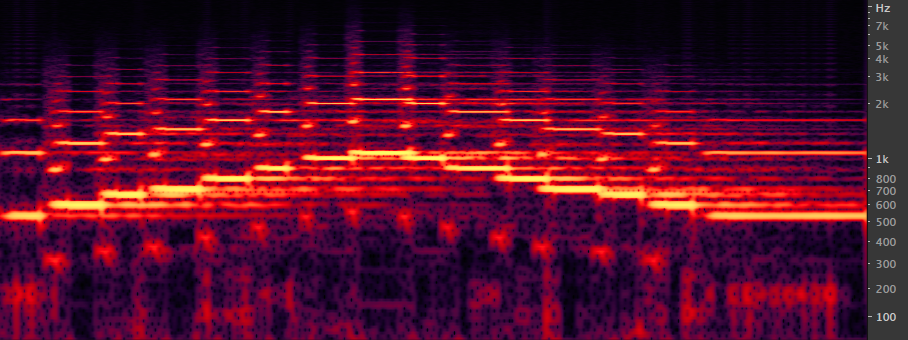
\includegraphics[width=\textwidth]{figures/spektrum-original.png}
	\caption{Frequenzspektrum eines Signals mit Watermark}
	\label{fig:spektrum-original}
\end{figure}

\begin{figure}[h]
	\centering
	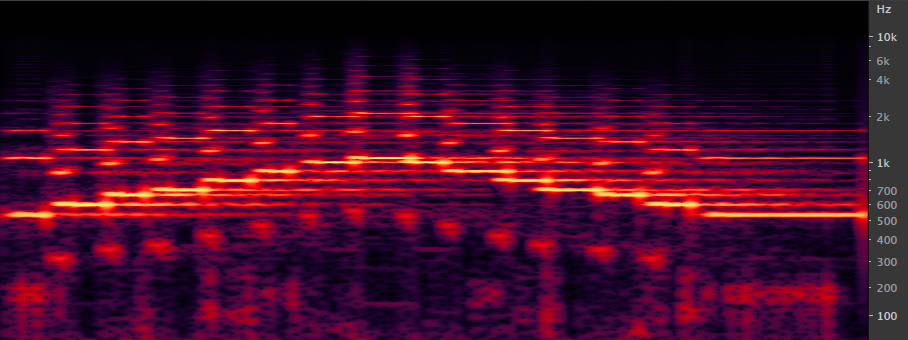
\includegraphics[width=\textwidth]{figures/spektrum-soundkarte.png}
	\caption{Frequenzspektrum nach DA- und AD- Wandlung}
	\label{fig:spektrum-soundkarte}
\end{figure}

Betrachtet man nun die Zusammensetzung jedes Bits genau, so wird man fündig. Wir erinnern uns: Jedes Bit ist durch die Energieniveaus ${E}_{1}$,${E}_{2}$ und ${E}_{3}$ der DWT-Koeffizienten\index{DWT-Koeffizienten} Subbänder\index{Subband} definiert. Der Bitwert $0$ oder $1$ ergibt sich aus dem Verhältnis der Energieddifferenzen $A$ und $B$ der Subbänder. Es zeigt sich, dass die Energieniveaus im Schnitt um den Wert $0.03$ abweichen. Daraus ergeben sich zwei beobachtete Effekte:

\begin{enumerate}
		
\item Die Sortierung zu ${E}_{min}$,${E}_{med}$ und ${E}_{max}$ der Subband-Energiewerte ${E}_{1}$,${E}_{2}$ und ${E}_{3}$ korreliert durch die Abweichung nicht mehr mit dem Ursprungssignal. Somit werden für die Berechnung von $A$ und $B$ falsche Bänder herangezogen, weswegen die Dekodierung folglich einen falschen Bitwert produziert. 
	
\item Auch wenn die Energieniveaus richtig sortiert werden, so kann es durch die Abweichungen dennoch dazu kommen, dass die korrekte Relation der Niveaudifferenzen $A$ und $B$ nicht mehr gegeben ist. Die Veränderung der Bänder kann beispielsweise ausreichen, dass bei einer kodierten $1$ im Dekodierprozess jedoch $A \ngtr B$ gilt, weswegen eine $0$ erkannt wird.
	
\end{enumerate}

An dieser Stelle sei noch darauf hingewiesen, dass die für dieses Testsignal gewählte analoge Übertragungsstrecke lediglich aus einem analogen Audiokabel bestand. Subjektive Hörtests lassen keinen merklichen Unterschied zwischen Originalsignal und übertragenem Signal feststellen. Die Belastung die das Signal daher durch diesen Übertragungskanal erfährt, ist denkbar gering. In Luft wäre diese beispielsweise viel massiver. 

Es zeigt sich also, dass die Energieniveaus der Bänder sehr fragil sind. Sie eignen sich demnach für einen Übertragungskanal der die niederfrequenten Energiepotenziale - wenn auch nur gering - verändern kann offensichtlich nicht. 